\chapter{プロット・グラフ}

\begin{abstract}
 
\end{abstract}

\section{Gnuplot}

定番中の定番.一番簡単かも.設定は自分の好きなようにやろうね.


\section{Ngraph}


%忘れちゃいけないよ


\section{Grapher}

グラフ描画

\begin{center}
 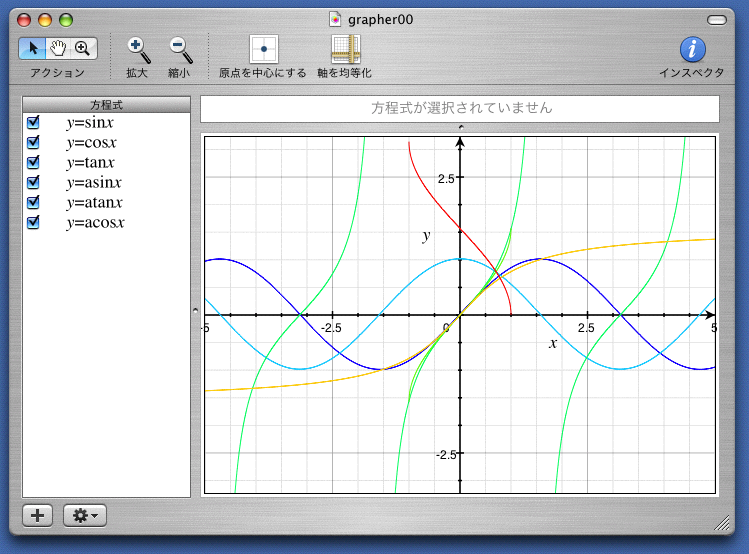
\includegraphics[scale=.4]{images/Grapher01}% 起動例
% ばっつばっつ関数を追加する.色も自動的に分けてくれる
 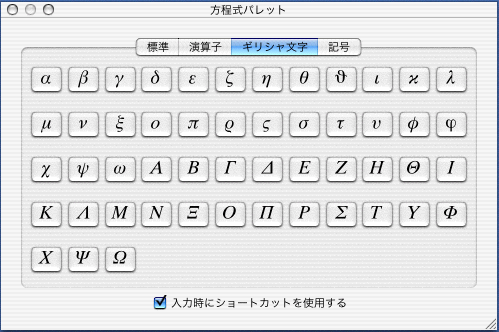
\includegraphics[scale=.4]{images/Grapher02}
% ばっつばっつ記号も使えるし,演算子,ギリシャ文字も用意されている
\end{center}

Grapher で作成したグラフの例

\begin{center}
 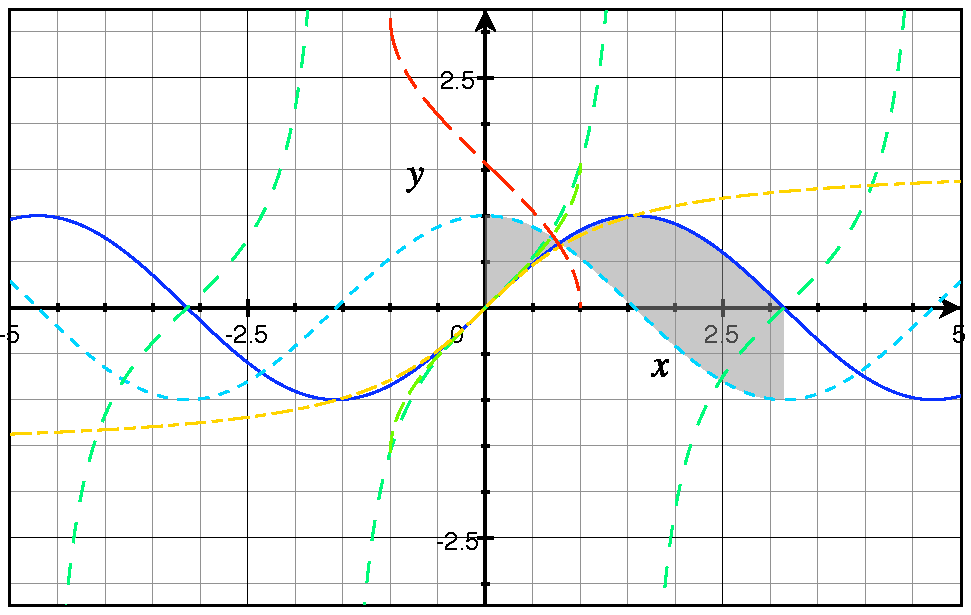
\includegraphics[scale=.4]{images/grapher00}
\end{center}


\section{R}

統計解析

\section{SciLab}

制御系

\section{Octave}

行列

